% -*- Mode:TeX -*-
% LaTeX template for CinC papers                   v 1.1a 22 August 2010
%
% To use this template successfully, you must have downloaded and unpacked:
%       http://www.cinc.org/authors_kit/papers/latex.tar.gz
% or the same package in zip format:
%       http://www.cinc.org/authors_kit/papers/latex.zip
% See the README included in this package for instructions.
%
% If you have questions, comments or suggestions about this file, please
% send me a note!  George Moody (george@mit.edu)
%
\documentclass[twocolumn]{cinc}
\usepackage{graphicx}
\begin{document}
\bibliographystyle{cinc}

% Keep the title short enough to fit on a single line if possible.
% Don't end it with a full stop (period).  Don't use ALL CAPS.
\title{The Title Should Be in This Format and Should Be \\
Clear Without Abbreviations or Period at End}

% Both authors and affiliations go in the \author{ ... } block.
% List initials and surnames of authors, no full stops (periods),
%  titles, or degrees.
% Don't use ALL CAPS, and don't use ``and'' before the name of the
%  last author.
% Leave an empty line between authors and affiliations.
% List affiliations, city, [state or province,] country only
%  (no street addresses or postcodes).
% If there are multiple affiliations, use superscript numerals to associate
%  each author with his or her affiliations, as in the example below.

\author {Ann Author$^{1}$, Charles D Coauthor$^{2}$ (note - no ``and", no periods, no degrees) \\
\ \\ % leave an empty line between authors and affiliation
 $^1$ Institution, City, Country (note - full address at end of paper) \\
$^2$  Second Institution, Other City, Country  }

\maketitle

% LaTeX inserts the ``Abstract'' heading in the proper style and
% sets the text of the abstract in italics as required.
\begin{abstract}

    Center the word Abstract and print it in Times New Roman 11-point size
    and in bold.

% Of course, you must insert blank lines
% between the paragraphs of your LaTeX input file, since this is the
% only way to indicate paragraph boundaries.  Make sure that no blank
% lines appear between paragraphs in the formatted output, however.)
% 
% 
    The abstract and all other text (except as indicated in
    Table~\ref{tab:font}) are printed in a 10-point size. The text of the
    abstract (and only the abstract) should be in italics. Begin all
    paragraphs with a 1 pica (4 mm, 1/6 inch) indentation.

    Do not add blank line spaces between paragraphs in the abstract or
    anywhere else in your article.

    The abstract with its heading should not be more than 100 mm long,
    which is equivalent to 25 lines of text. Leave 2 line spaces at the
    bottom of the abstract before continuing with the next heading.

\end{abstract}
% LaTeX inserts the extra space here automatically.

\section{Introduction}
% Section numbering is automatic.  The examples on the next page
% illustrate how to make subsections.

Leave one line space above and below all headings from now on.

Number your sections (e.g., 1.  1.1.  1.2.  - note the decimal points) as
illustrated. Start the text of section headings after a 12 mm (0.5 inch)
tab.

% LaTeX converts the reference tag ('WP-89') into a reference number,
% which it inserts in the formatted text as '[1]'.  If you use BibTeX
% to handle references, BibTeX finds a reference with the tag 'WP-89'
% in 'refs.bib', and inserts that reference into the ``References''
% section in CinC style.
% 

\subsection{Print font}

Please use Times New Roman font. Use of this font by all authors ensures
that our papers are produced consistently with a professional appearance.


 \subsection{ Print size}  

Follow the information given in Table 1 for all font print sizes and styles.

\section{Title block}
 
On the first page, the title, authors, and institution(s) should be
positioned and aligned as above.

\subsection{Title} 
 
Do not use abbreviations in the title and keep to one or two
lines. Remember that the title should be easily understood when cited as a
reference in another publication. Make sure the title is centered. Note the
use of capital letters, as shown in the example above. Do not place a
period at the end of the title.

\subsection{ Author line}  
 
If it is essential to link authors to different institutions, use a small
superscript at the end of each family name and link to each institution. No author degrees should be
included. No periods should appear in the author line.

 \subsection{ Institution address} 

 This address identifies the institution(s). It is not a postal address and
 should not contain postal or zip codes. A full postal address is given at
 the end of the paper under `Address for correspondence'. Do not put line
 spaces between address lines or use a period at the end.
 
 \section{ Tables and figures}
\subsection{Tables} 
\vspace{-4 mm}
\begin{table}[htbp]
\caption{\label{tab:font} Print sizes for different parts of the paper.}
\vspace{4 mm}
\centerline{\begin{tabular}{lcr} \hline\hline
Text    & Point size    & Type \\ \hline
Title   & 14 point      & Bold \\
Author line     & 12 point      & \\
Institution line        & 12 point      & \\
Abstract heading        & 11 point      & Bold \\
All other headings      & 12 point      & Bold \\
Abstract text   & 10 point      & Italic \\
References and address  & 9 point       & \\
All other text  & 10 point      & \\ \hline\hline
\end{tabular}}

\end{table}

Keep \ the layout of \ tables simple. Avoid  heavy lines and boxes.

\subsection{ Figures}   

Figures can fit across both columns if necessary. Include all figures, with
captions, in the text document at their desired locations, i.e., not at the
end. To make sure that all labels are legible, use at least 9-point
font. Use a line thickness of at least 0.5 mm in the body of the figure.

\begin{figure}[h]
%\centering
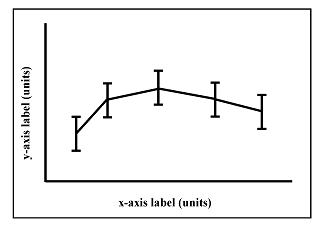
\includegraphics[width=7.9cm]{fig/graph.png}
\caption{Put the figure legend here, at the bottom, clearly describing the
  figure.}
\label{FIGURA1}
\end{figure}

Leave a line space after a figure legend. Be cautious with background
colors in figures because they can make printed figures hard to read.

\section{Final page}

The text on the final page should be arranged so that both columns are
approximately the same length.

\balance

\section{Style of references}     

All references should be included in the text in square brackets in their
order of appearance, e.g., \cite{tag}, \cite{tag,ito}, or
\cite{tag,ito,fardel,buncombe}. In the reference list, use the Vancouver
style (see IEEE Transactions on Biomedical Engineering or Annals of
Biomedical Engineering). The main goal is to be consistent in your
formatting of references.

References to \emph{Computers in Cardiology} (or \emph{Computing in
  Cardiology}) proceedings should include the volume and page numbers,
unless no page numbers were included (post-2016). Check the style in the
examples below.


\section{ Final checks }     
 
Print this template without resizing or centering and compare with your
final paper to ensure that you have not accidentally changed margins and
layout.


\section*{Acknowledgments}  
% This section is not numbered.
% 
Give any acknowledgments here.


% LateX generates the ``References'' heading automatically and switches
% to 9 point type for the bibliography.  Please  use BibTeX and
% follow the examples in the sample 'main.bib' file to enter your references.
\bibliography{main}

% If you don't use BibTeX (why not?) , comment out or remove the previous
% line, and uncomment the following lines up to the ``}\end{bibliography}''
% line below:
%\begin{thebibliography}{99}{ %\small
% \bibitem{tag} (General form) J. K. Author, ``Name of paper,''
%   \emph{Abbrev. Title of
%   Periodical}, vol. x, no. x, pp. xxx--xxx, Abbrev. Month, year. 

% \bibitem{ito}  M. Ito et al., ``Application of amorphous oxide TFT to
%   electrophoretic display,'' \emph{J. Non-Cryst. Solids}, vol. 354, no. 19,
%   pp. 2777--2782, Feb. 2008.
  
% \bibitem{fardel}  R. Fardel, M. Nagel, F. Nuesch, T. Lippert, and
%   A. Wokaun, ``Fabrication of organic light emitting diode pixels by
%   laser-assisted forward transfer,'' \emph{Appl. Phys. Lett.}, vol. 91,
%   no. 6, Aug. 2007, Art. no. 061103.
  
% \bibitem{buncombe} J. U. Buncombe, ``Infrared navigation Part I: Theory,''
%     \emph{IEEE Trans. Aerosp. Electron. Syst.}, vol. AES-4, no. 3,
%     pp. 352--377, Sep. 1944.
      
% Uncomment the following line if you are not using BibTeX.
%}\end{thebibliography}


% LaTeX inserts the ``Address for correspondence'' heading.
\begin{correspondence}
My Name\\
My Full postal address\\
My E-mail address
\end{correspondence}

\end{document}

